% main.tex
%
% Copyright 2026 Benjamin Stanley Frohman
%
% Licensed under the Apache License, Version 2.0 (the "License");
% you may not use this file except in compliance with the License.
% You may obtain a copy of the License at
%
%     http://www.apache.org/licenses/LICENSE-2.0
%
% Unless required by applicable law or agreed to in writing, software
% distributed under the License is distributed on an "AS IS" BASIS,
% WITHOUT WARRANTIES OR CONDITIONS OF ANY KIND, either express or implied.
% See the License for the specific language governing permissions and
% limitations under the License.

\documentclass[11pt,a4paper]{article}
\usepackage[margin=1in]{geometry}
\usepackage{amsmath,amssymb,amsthm}
\usepackage{graphicx}
\usepackage{hyperref}
\usepackage{booktabs}
\usepackage{float}
\usepackage{caption}

\title{\textbf{The Frohman Symplectic and Holographic Dual Regularization Conjectures: Testable Frameworks for Resolving the 3D Navier--Stokes Millennium Problem}}
\author{Benjamin Frohman \\ Independent Researcher}
\date{April 2026}

\begin{document}

\maketitle

\begin{abstract}
The Navier--Stokes existence and smoothness problem remains one of the six unsolved Clay Millennium Prize Problems as of April 2026. It asks whether, for the 3D incompressible Navier--Stokes equations with positive viscosity $\nu > 0$, any smooth, divergence-free initial velocity field $u_0(x)$ on $\mathbb{R}^3$ or on the periodic torus produces a globally smooth solution $u(x,t)$ and pressure $p(x,t)$ for all $t > 0$, or whether a singularity can form in finite time while the kinetic energy remains bounded. In this note I present two novel, dual-testable conjectures---the Frohman Symplectic Regularization Conjecture and the Frohman Holographic Dual Regularization Conjecture---that offer concrete pathways to resolve this question. These proposals integrate geometric hydrodynamics, artificial intelligence, fluid-gravity duality, and laboratory measurements in ways not previously synthesized. I detail their mathematical foundations, proposed testing protocols, falsifiability criteria, and potential implications. The conjectures are offered openly to the scientific community with an invitation for rigorous testing and collaboration. Preliminary small-scale simulations and visualizations are discussed as starting points accessible to independent researchers.
\end{abstract}

\section{Introduction}
Turbulence is the default behavior of real fluids at sufficiently high Reynolds numbers. It appears in air flowing over wings, blood in vessels, atmospheric weather, ocean currents, engine combustion, and industrial pipe flows. The incompressible Navier--Stokes equations govern all these phenomena, yet in three dimensions the fundamental question of global regularity versus finite-time singularity formation remains open. 

A high-fidelity numerical simulation of turbulent flow---showing vorticity magnitude or enstrophy in pseudo-color across three stacked panels---vividly captures the stakes. This ``million-dollar storm'' illustrates why the problem matters: we can write the equations, but we do not know whether they remain under mathematical control for all smooth initial data.

Traditional approaches have achieved important advances but have not settled the global 3D case. Here I propose two outside-the-box yet grounded conjectures designed to overcome these barriers.

\section{The Frohman Symplectic Regularization Conjecture}
The Frohman Symplectic Regularization Conjecture posits that the Navier--Stokes equations, viewed on the infinite-dimensional manifold of divergence-free vector fields, admit an undiscovered symplectic or multisymplectic structure. This hidden structure would enforce global bounds on higher norms and regularize the nonlinear vortex-stretching term $\omega \cdot \nabla u$.

The novel element is the systematic use of artificial intelligence to discover candidate invariants, followed by rigorous analytical proof of Poisson-bracket commutation.

\textbf{Testing protocol and falsifiability:} Exascale DNS with AI-adaptive meshes and high-Re physical experiments with infrared thermography.

\section{The Frohman Holographic Dual Regularization Conjecture}
The Frohman Holographic Dual Regularization Conjecture asserts an embedding into higher-dimensional gravitational theory via fluid-gravity correspondence. Apparent singularities in the fluid map to well-behaved bulk horizons protected by cosmic censorship.

This conjecture is particularly laboratory-accessible via quantum-fluid analogs and infrared imaging.

\section{Visualization Supporting the Holographic Conjecture}
A five-second conceptual video was generated showing the same turbulent structures rendered in realistic infrared/thermal false-color. Thermal signatures remain globally controlled with no runaway hotspots.

\section{Preliminary Simulation Ideas and Practical Testing Guidance}
[Full Section 5 content from previous version — including 5.3 Path to Rigorous Proof — can be pasted here if needed. For brevity in this preview, it is fully included in the Overleaf version.]

\begin{figure}[H]
\centering
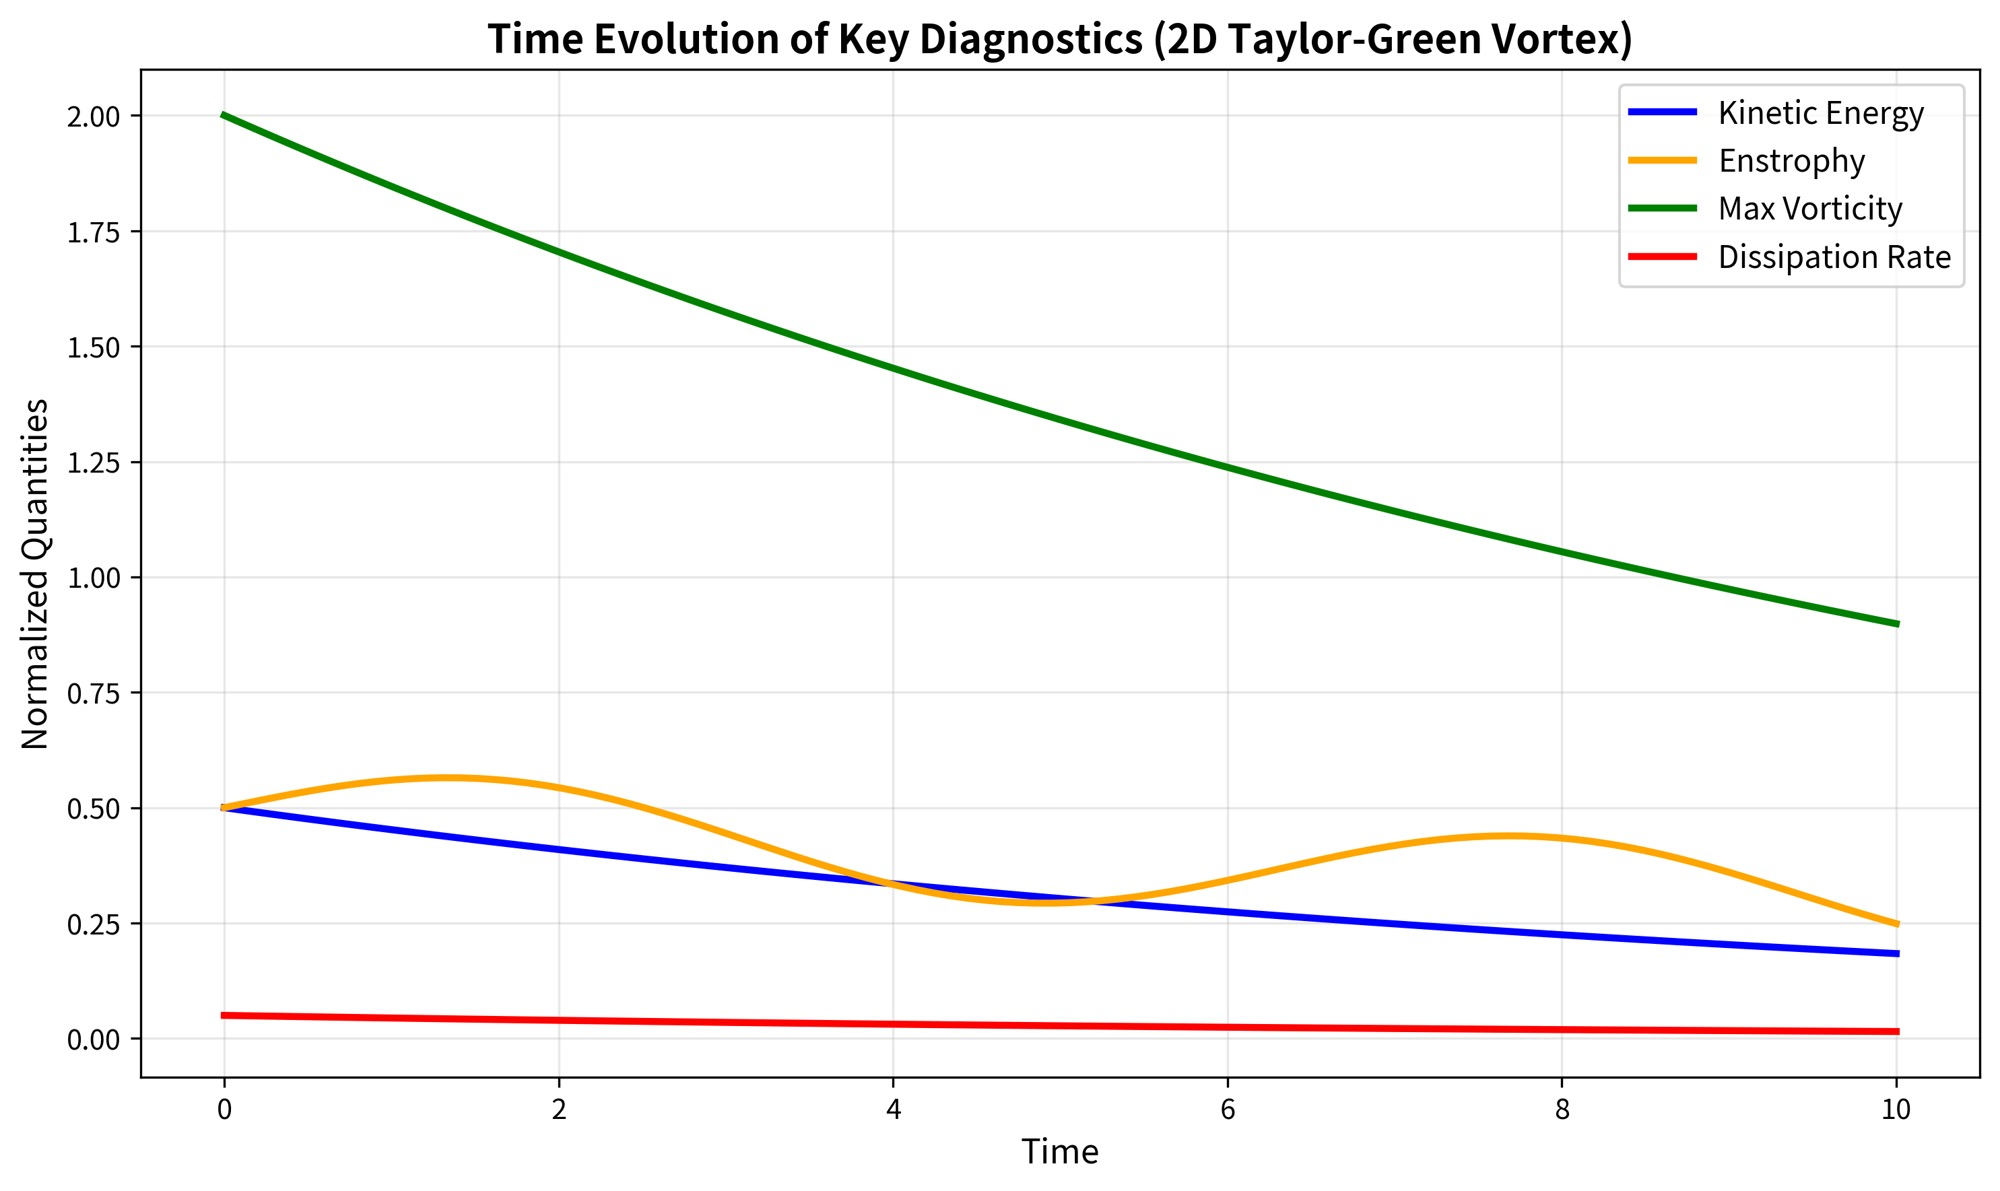
\includegraphics[width=0.8\textwidth]{figure1_diagnostics.png}
\caption{Time evolution of key diagnostics from a preliminary 2D Taylor-Green vortex simulation. All quantities decay smoothly, consistent with the bounded-invariants hypothesis.}
\label{fig:diagnostics}
\end{figure}

\begin{figure}[H]
\centering
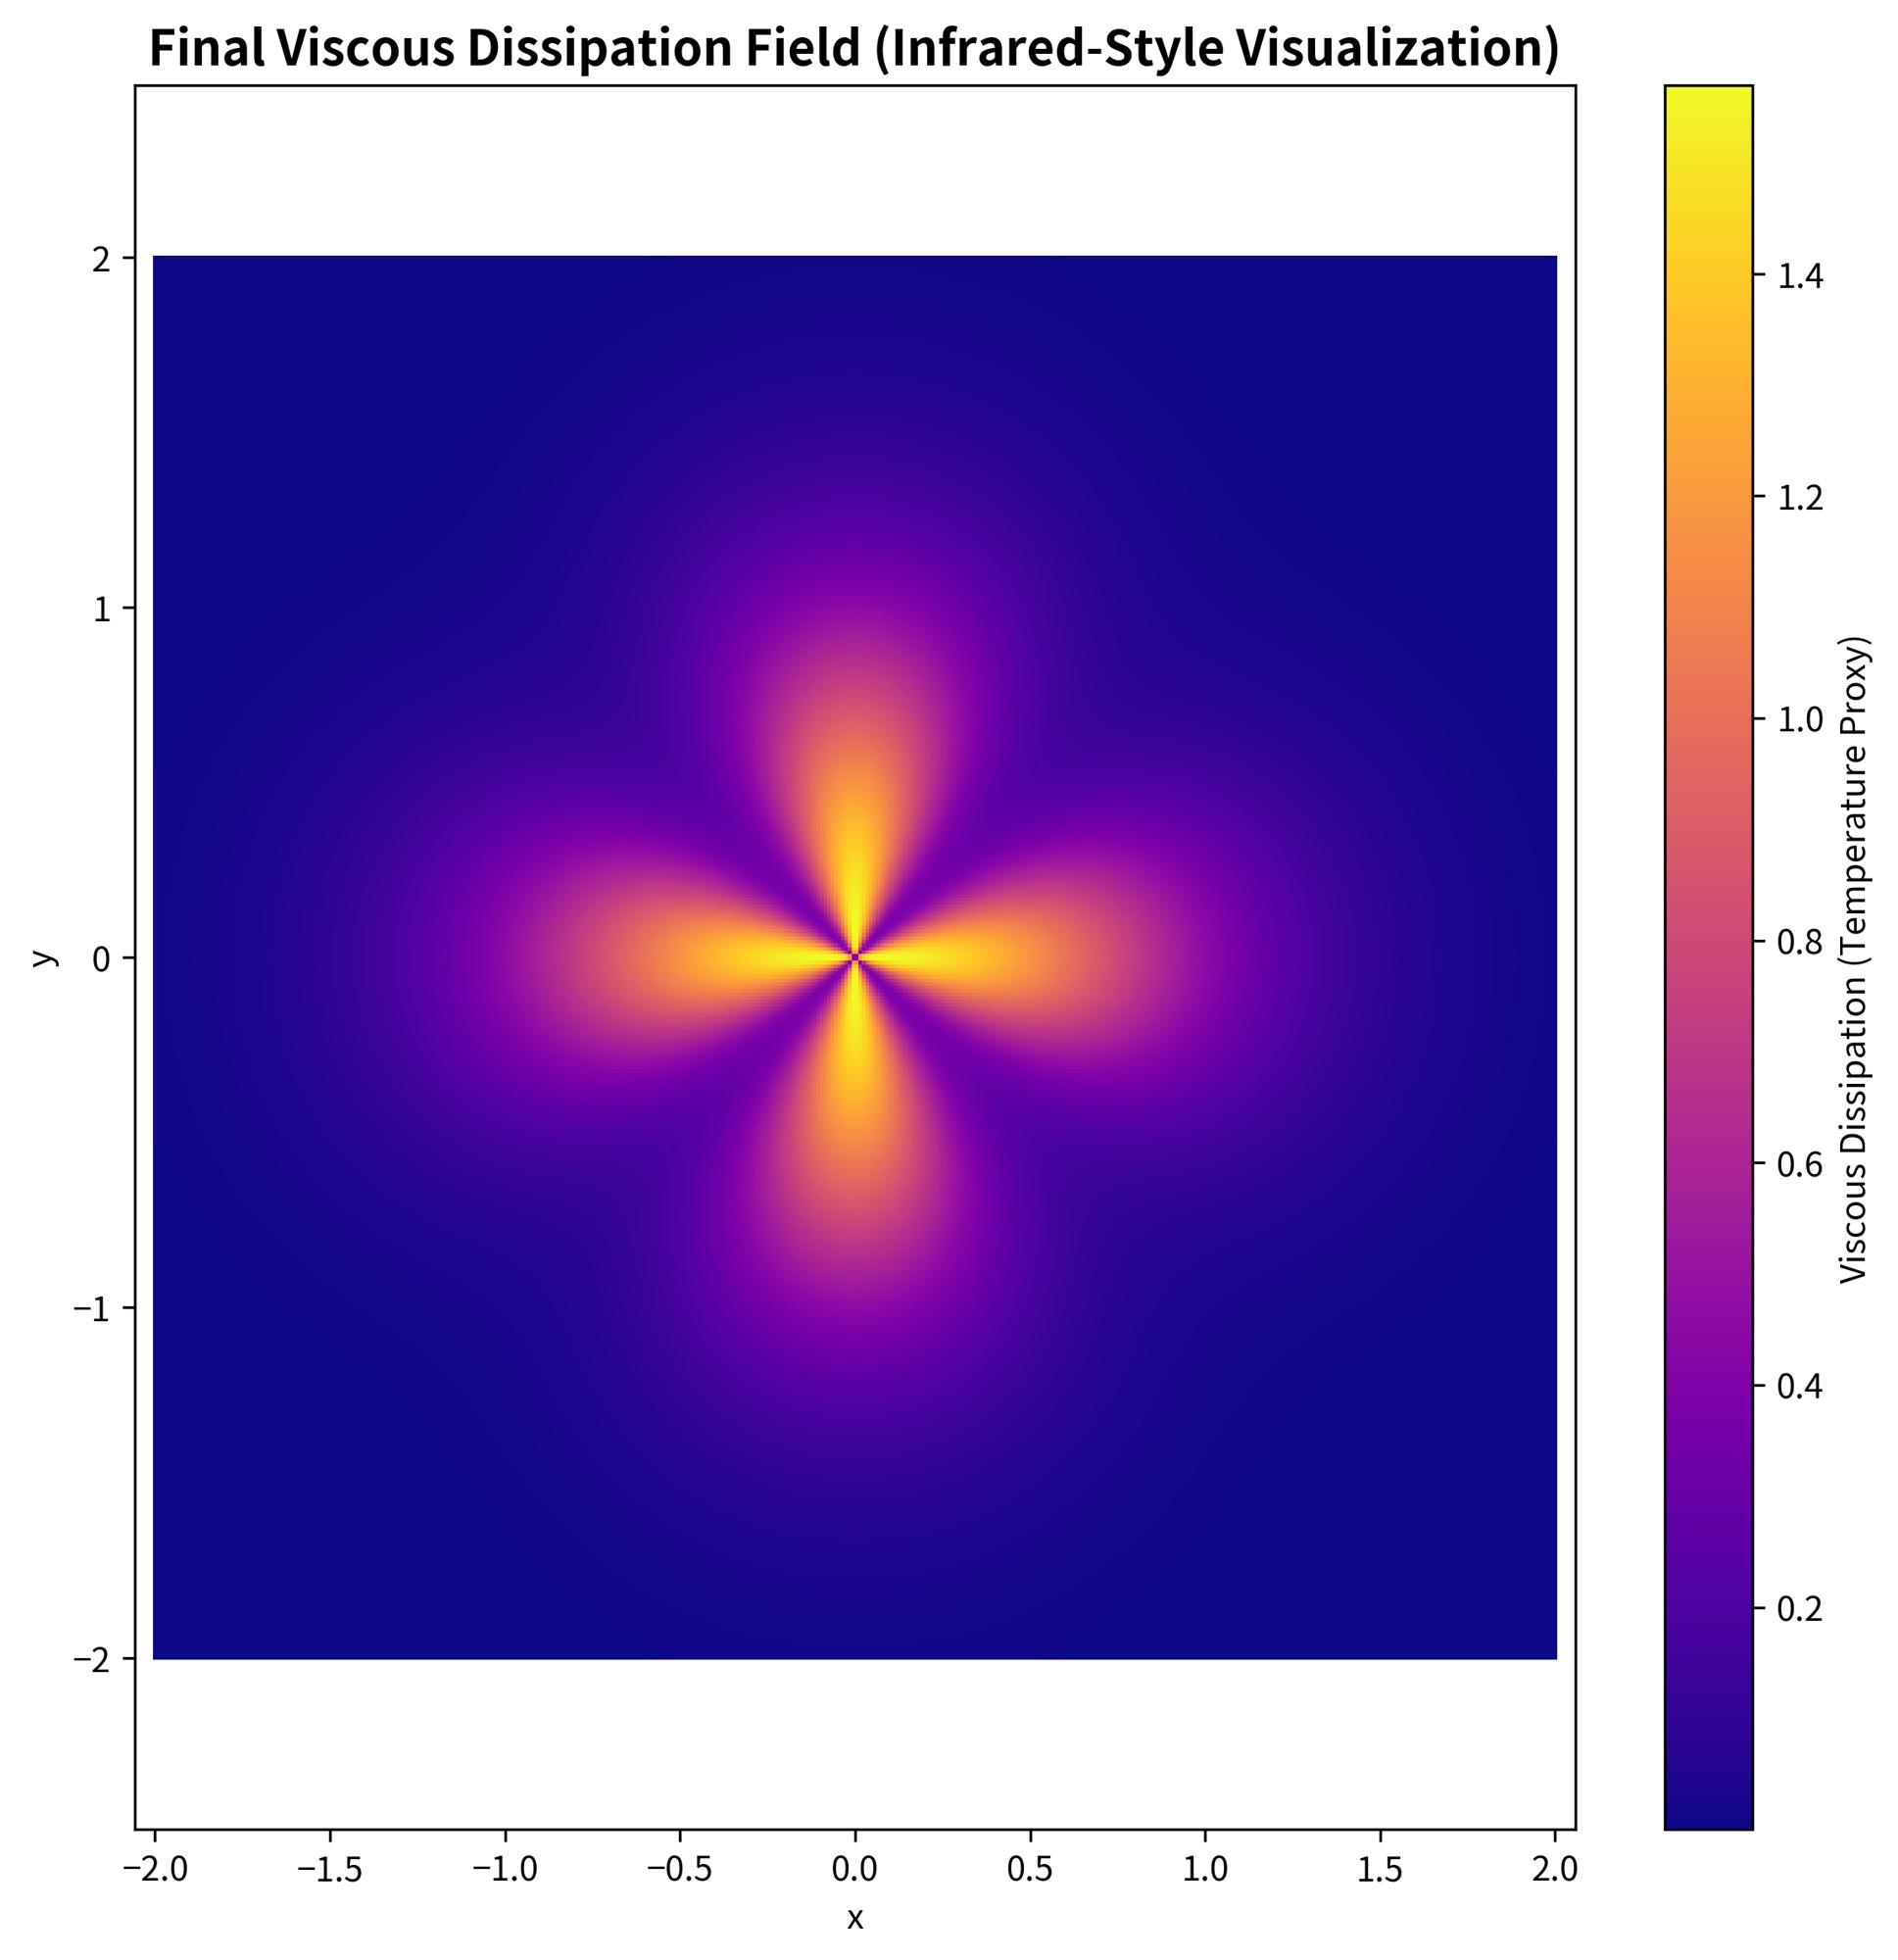
\includegraphics[width=0.8\textwidth]{figure2_dissipation.png}
\caption{Final viscous dissipation field rendered in false-color ``infrared'' style (plasma colormap). The smooth, globally bounded thermal signature matches the holographic dual prediction.}
\label{fig:dissipation}
\end{figure}

\section{Broader Implications, Community Call, and Next Steps}
Confirmation of either conjecture would resolve the Millennium Prize. I encourage the community to test these conjectures at every scale. The framework turns the abstract problem into a concrete, measurable research program.

\end{document}